
Inicialmente, buscou-se compreender os requisitos do escalonador através de entrevistas com outros alunos

\section{Sistema de Escalonamento do BioNimbuZ}

\begin{figure}[htbp]
	%	\centerline{\includegraphics[scale=0.04]{img/EscalonadorProposto.png}}
	\centerline{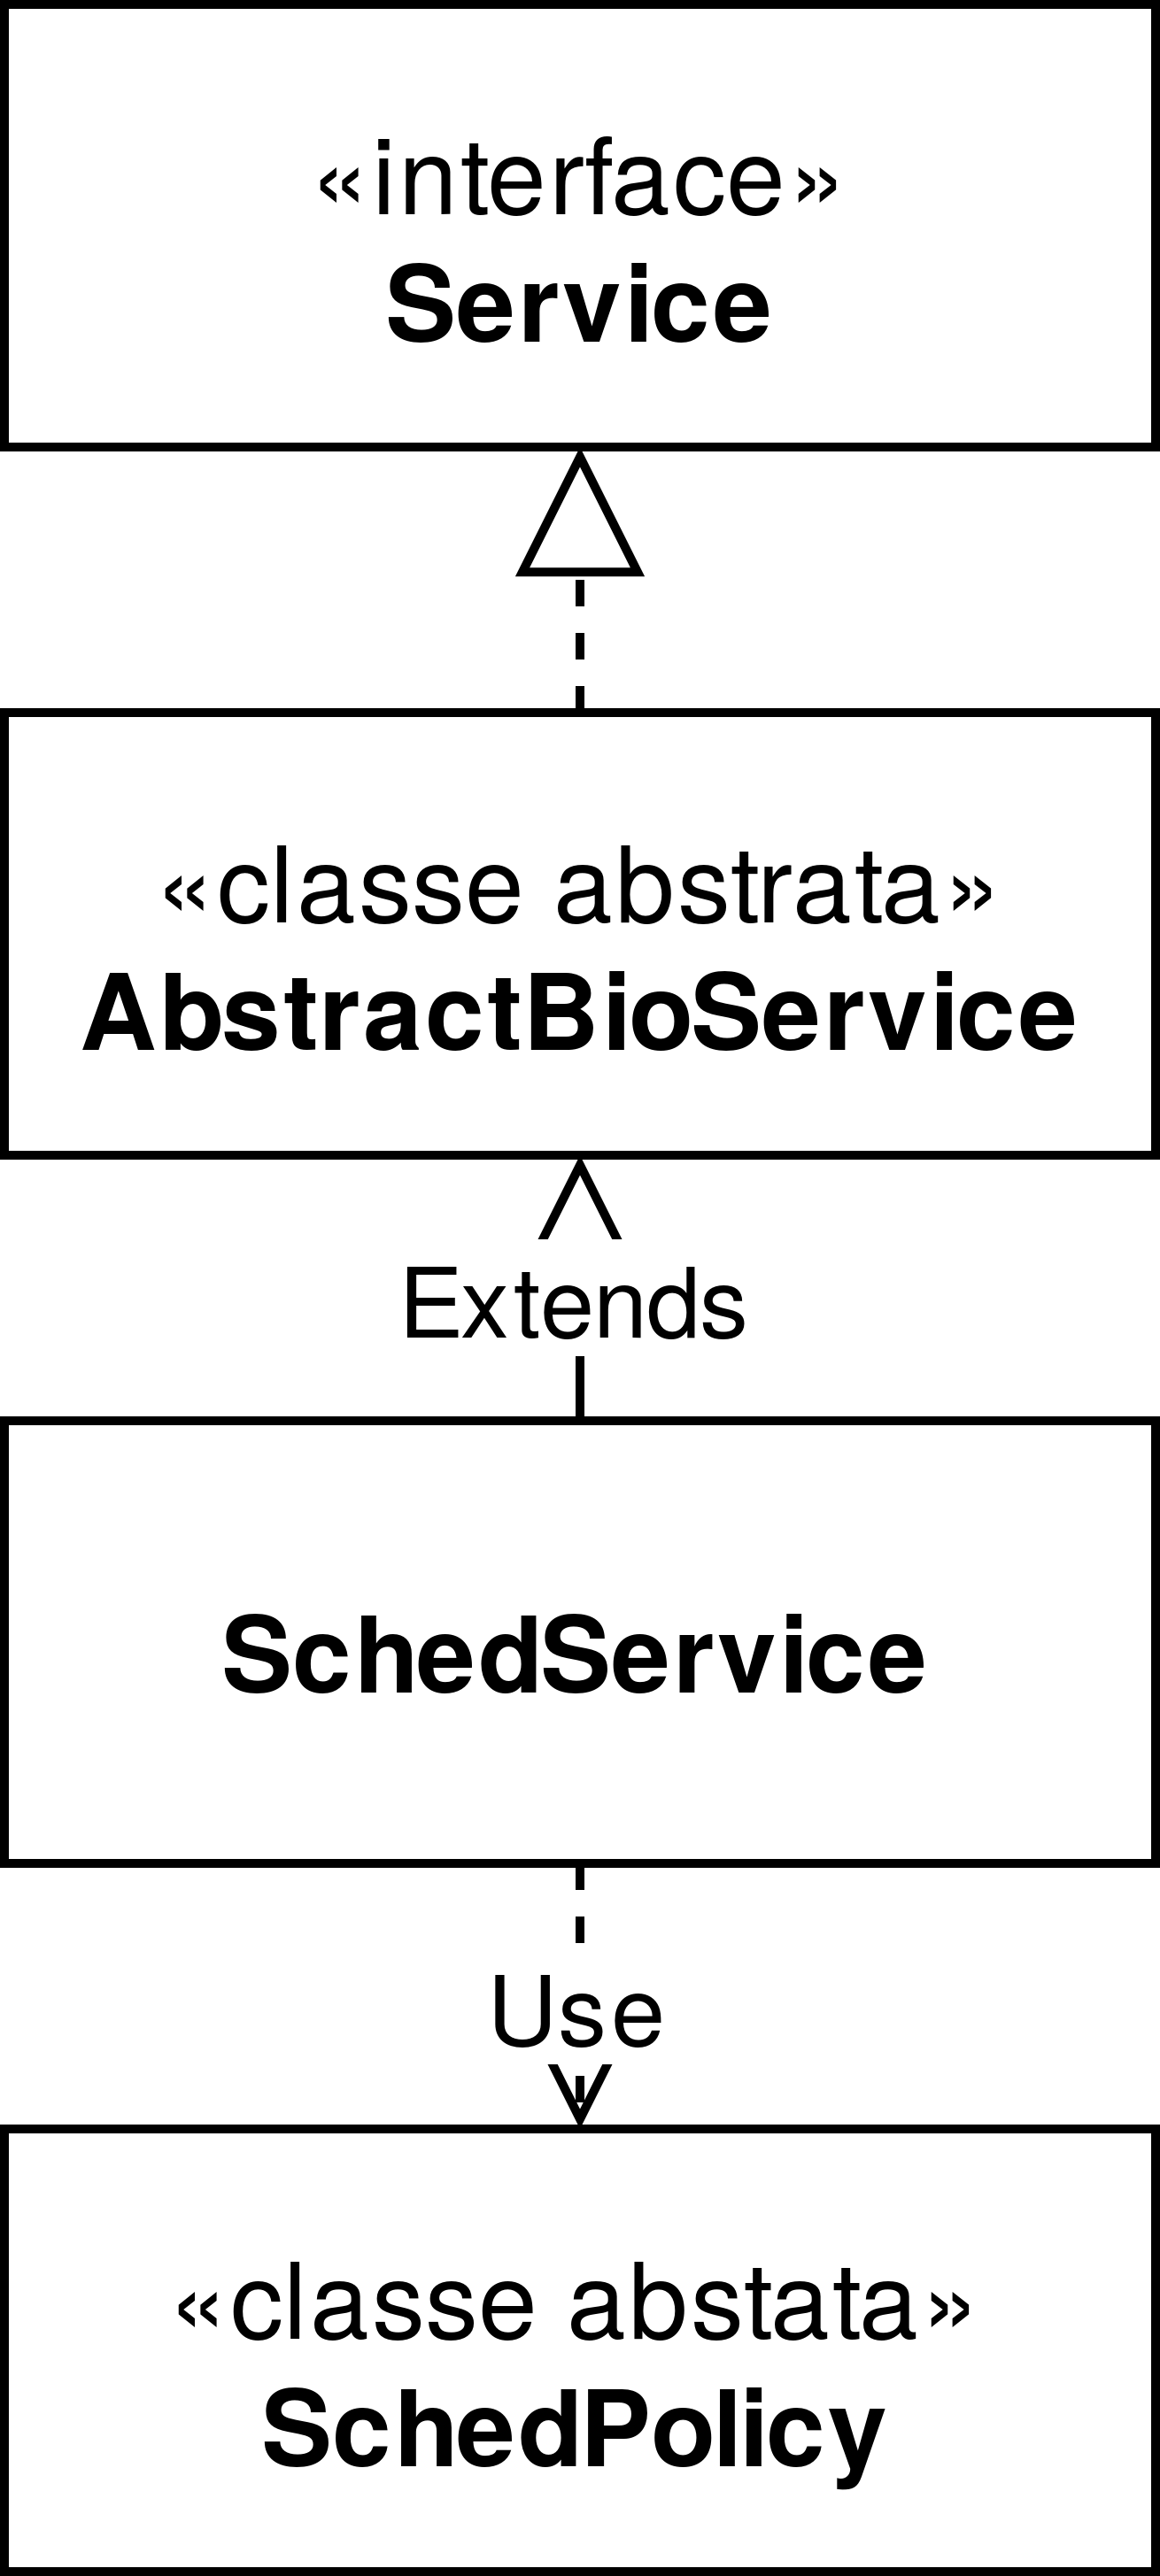
\includegraphics[width=3cm]{img/SubsistemaDeEscalonamento.png}}
	\caption{Subsistema de Escalonamento}
	\label{SubsistemaDeEscalonamento}
\end{figure}


O escalonamento é implementado como um serviço, como mostrado na figura \ref{SubsistemaDeEscalonamento}. A interface \textit{services} define métodos para inicialização, término de serviços e métodos para comunicação com o \textit{Zookeeper}. A classe \textit{AbstractBioService} define funcionalidades comuns aos serviços do BioNimbuZ, em especial comunicação entre as máquinas que compõem a plataforma e o padrão de projeto \textit{observer}, utilizado para notificação de eventos. A classe \textit{SchedService} é a resposável por prover o serviço de escalonamento em si, entretanto, para permitir a existência de várias políticas de escalonamento, internamente ela utiliza instâncias da classe abstrata \textit{SchedPolicy}, que implementam cada uma das distintas políticas de escalonamento existentes.


\begin{figure}[htbp]
	\centerline{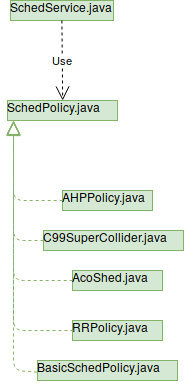
\includegraphics[scale=0.7]{img/ArquiteturaAntes.png}}
	\caption{Arquitetura do Subsistema de Escalonamento}
	\label{ArquiteturaAtual}
\end{figure}

Essas políticas de escalonamento são implementadas através da definição dos seguintes métodos herdados de \textit{SchedPolicy}:
\begin{itemize}
%	\item \textit{schedule}, que recebe como arguento uma lista de \textit{Jobs} para ser escalonado e retorna um mapeamento de \textit{Job} para um conjunto de máquinas as quais realizarão a computação.
	\item \textit{schedule}, que realiza o escalonamento inicial propriamente dito;
	\item \textit{relocate}, o qual realoca um processamento que está e execução;
	\item \textit{cancelJobEvent}, cujo objetivo é reportar ao escalonador o cancelamento de um \textit{Job};
	\item \textit{jobDone}, que informa ao escalonado que um \textit{Job} terminou.
\end{itemize}


Por motivos de familiaridade com a linguagem de programação, o escalonador proposto foi implementado em C++. Para ter compatibilidade com o resto do software, classes auxiliares, como a que representa os \textit{Jobs} e as \acrshort{VM}s instanciáveis tiveram equivalentes escritos em C++. Além disso, dois outros problemas surgiram: Como iniciar o escalonador C++ e como ele deve se comunicar com o resto da plataforma. O primeiro problema foi resolvido através de pesquisa na \acrfull{API} do Java, utilizando as classes \textit{Runtime}\cite{JavaRuntime} e \textit{Process}\cite{JavaProcess} é simples executar comandos de terminal, o que permite execução da parte C++ do escalonador.

O problema da comunicação do C++ com o Java é mais difícil, pois há várias formas de fazer. Por exemplo o uso de classes \textit{wrappers} que usam \textit{handles}, que são objetos cujos objetivos é manipular estruturas que não são nativas da linguagem\cite{CppJavaHandle}. Uma outra forma documentada é através do uso do \acrfull{JNI}, que é uma outra forma existente que faz possível através do uso de \textit{handles} chamar código C++ num programa Java\cite{CppJavaJNI}, também existem variações deste método utilizando bibliotecas que busca simplificar de alguma forma o gerenciamento do \textit{handle}. Como as formas pesquisadas para fazer tal comunicação aparentam não chegar a um consenso, decidiu-se então utilizar formas mais genéricas de comunicação entre processos, onde então surgiu a ideia de usar \textit{sockets} para fazer a comunicação.
